%These are the variables you change to manipulate the header.
\newcommand{\School}{Academic Institution}
\newcommand{\Class}{Class Title}
\newcommand{\Assignment}{Assignment Title}
\newcommand{\Name}{Your \textsc{Name}}
\newcommand{\Professor}{Professor's \textsc{Name}}
%This can be left as `\today`, which prints today's date upon compile, or it can be changed to reflect a due-date.
\newcommand{\Duedate}{\today}
%The document font size and style go here. Options include: article, report, book, letter, and many more. See the [Wikibooks](https://en.wikibooks.org/wiki/LaTeX/Document_Structure#Document_classes).
\documentclass[11pt]{article}
%Define paper dimensions...
\usepackage{geometry}
\geometry{letterpaper}
%and begin including essential packages. These give us advanced math typesetting...
\usepackage{amssymb,amsmath,cancel}
%... some useful utilities for figures...
\usepackage{caption, subcaption}
%... a nicer header...
\usepackage{setspace}
%... and reduced margins by default.
\usepackage{fullpage}
%Additionally, this one lets me use `\lipsum` to render Lorem Ipsum for this demo.
\usepackage{lipsum}
%Tikz is a powerful package for graphics rendering, which we cover in a bit.
\usepackage{tikz}		% for graphics
\usetikzlibrary{decorations.pathreplacing, calc}
\usetikzlibrary{snakes,shapes,decorations.text}
%These are custom derivative macros which I was given by Lily Chen (MIT). They are used with two arguments (`\d{y}{x}`), and print fractions of the form dy/dx. More on that later.
\let\underdot=\d
\renewcommand{\d}[2]{\frac{d #1}{d #2}}
\newcommand{\dd}[2]{\frac{d^2 #1}{d #2^2}}
\newcommand{\pd}[2]{\frac{\partial #1}{\partial #2}}
\newcommand{\pdd}[2]{\frac{\partial^2 #1}{\partial #2^2}}
%Also, this is pretty useful.
\newcommand{\degrees}{\ensuremath{^\circ}}
\begin{document}
  %This prints the title page, which is informed by the variables from the first section. One might play with spacing and font sizes.
  \begin{titlepage}
    \newcommand{\HRule}{\rule{\linewidth}{0.5mm}}
    \center
    \textsc{\LARGE \School}\\[1.5cm]
    \textsc{\Large \Class}\\[0.3cm]
    \HRule \\[0.4cm]
    { \huge \bfseries \Assignment}\\[0.1cm] 
    \HRule \\[1.5cm]
    \begin{minipage}{0.4\textwidth}
      \begin{flushleft} \large
        \emph{Author:}\\
        \Name
        \end{flushleft}
        \end{minipage}
        ~
        \begin{minipage}{0.4\textwidth}
        \begin{flushright} \large
        \emph{Course Instructor:} \\
        \Professor \\
      \end{flushright}
    \end{minipage}
      \\[1cm]
    {\large \Duedate}\\[3cm]
    \vfill
  \end{titlepage}

  \newpage 
  \begin{abstract}
    \lipsum[1-3]
  \end{abstract}

  \newpage 
  %This auto-generates based on the `\section`s and `\subsection`s and `\subsubsection`s in the paper.
  \tableofcontents
  %Similarly, this auto-generates based on the `figure`s. There is a corresponding one for tables.
  \listoffigures

  \newpage
  %Sections are denoted with `\section{arg}`, where the `arg` is the title.
  \section{Section}
  Cras nibh. Morbi vel justo vitae lacus tincidunt ultrices. Lorem ipsum dolor sit amet, consectetuer adipiscing elit.
  %Sections can contain nested subsections, down to four-deep. These are called `\subsection`s, etc.
  \subsection{Derivation}
  Fusce mauris. Vestibulum luctus nibh at lectus. Sed bibendum, nulla a faucibus semper, leo velit ultricies tellus, ac venenatis arcu wisi vel nisl. 
  %Math may be written inline, when nested between two `$dollar signs$`: 
  Quisque ullamcorper placerat ipsum. $x^2$. Et, $y = 10\degrees$.
  Praesent enim elit, rutrum at, molestie non, nonummy vel, nisl. Ut lectus eros, malesuada sit amet, fermentum eu, sodales cursus, magna.
  %Or it can be printed formally, centered on a page.:
  $$ x^2 + y^2 = z^2 $$
  Donec eu purus. Quisque vehicula, urna sed ultricies auctor, pede lorem egestas dui, et convallis elit erat sed nulla. Donec luctus. Curabitur et nunc.
  %We also use align environments to create continuity. Use the `&` alignment mark to align the `=` signs of each equation
  \begin{align*}
    z^2 &= x^2 + y^2 \\
    z &= \sqrt{x^2 + y^2} \\
    %This is a custom macro defined above � `\d{x}{y}` won't work everywhere.
    \dot z = \d{z}{t} &= \d{\sqrt{x^2+y^2}}{t} = \d{}{t}\sqrt{x^2+y^2}
  \end{align*}
  %Figures and tables can be referred to from anywhere. Use a `\label` *below* each caption and `\ref`er to that label by name elsewhere.
  See Figure~\ref{named_schematic} on pp.~\pageref{named_schematic}.
  %`figure` environments can be given placement instructions, such as on their own page, or at the top or bottom of a page. Use `\begin{figure}[p]`, or `[b]`, or `[t]`.
  \begin{figure}[p]
    \begin{center}
      %`tikzpicture` environments contain `TikZ` script, which is slightly different. Lines must be terminated with a `;` semicolon, and variables may be used. For more on `TikZ`, see the [TikZ primer](https://en.wikibooks.org/wiki/LaTeX/PGF/TikZ).
      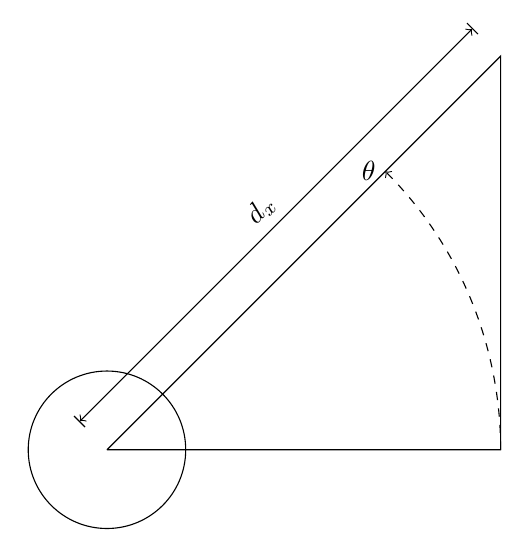
\begin{tikzpicture}
        \coordinate(O) at (0,0);
        \coordinate(A) at (5,0);
        \coordinate(B) at (5,5);
        %coordinates can be defined and then used symbolically. One could also write `\draw (0,0)--(5,0)--(5,5)--(0,0);` and achieve the same result.
        \draw (O)--(A)--(B)--(O);
        \draw (O) circle [radius=1];
        %Drawing lines requires points `(A)--(B)`. Arrow shape on both ends can be specified symbolically as a first option.
        %Here we use the `calc` library to add coordinates (`($(A)+(B)$)`). In this case, our second point is defined in polar (`(angle:radius)`) coordinates, rather than cartesian. 
        %Similarly, we mount a label (`node`) along the line, with some options. Its text is given by the contents of `{ }`, which can be any valid LaTeX.
        \draw [|<->|] ($(O)+(135:0.5)$) -- ($(B)+(135:0.5)$) node[midway, above, sloped] {$d_x$};
        %We can provide other line options, like `dashed` or `red` to the line. 
        %This is an `arc` command, which begins at a point (`A`) and follows an arc counterclockwise from angle `0` to angle `45` with radius `5`. Upon termination, we anchor to this node a text box at its east face.
        \draw [->, dashed] (A) arc ( 0 : 45 : 5) node[anchor=east] {$\theta$};
      \end{tikzpicture}
    \end{center}
    %Captions should go after figures, just before the figure close tag (`\end{figure}`).
    \caption{Schematic with Title}
    %Labels *must* go after captions.
    \label{named_schematic}
  \end{figure}
\end{document}
